%% ============================================================
%% COMPLETE UNIFIED IEEE PAPER — latexcode_final.tex
%% A Quantitative Framework for Options Mispricing Detection
%% Using EGARCH-Based Volatility Forecasting and Regime-Aware
%% Pricing in the NIFTY 50 Options Market
%% ============================================================

\documentclass[journal]{IEEEtran}

\usepackage{cite}
\usepackage{amsmath}
\usepackage{amssymb}
\usepackage{array}
\usepackage{tabularx}
\usepackage{booktabs}
\usepackage{float}
\usepackage{graphicx}
\usepackage{hyperref}

\hyphenation{op-tical net-works semi-conduc-tor}

\begin{document}

\title{A Quantitative Framework for Options Mispricing Detection Using
EGARCH-Based Volatility Forecasting and Regime-Aware Pricing in the
NIFTY~50 Options Market}

\author{%
  \IEEEauthorblockN{Heet Kothari, Meet Mehta, Shaurya Jain, Pramod Bide}
  \IEEEauthorblockA{}%
}

\markboth{}%
{Kothari \MakeLowercase{\textit{et al.}}: Quantitative Framework for
Options Mispricing Detection in NIFTY~50}

\maketitle

\begin{abstract}
The framework detects model-implied option pricing deviations; a claim
of economic mispricing is reserved for signals satisfying the
validation hierarchy in Section~V-M.

Quantitative pricing uses the HMM's filtered posterior probability
vector and posterior-weighted VRP; any dominant-regime label is
reserved for presentation or human-readable recommendations.

Options are commonly priced using the Black--Scholes model, where
implied volatility serves as the primary input for estimating
theoretical option values. However, implied volatility is itself
derived from market prices, creating a circular dependency when the
same contract's implied volatility is used both to construct and
evaluate its theoretical value. This paper presents a quantitative
framework for detecting model-implied option pricing deviations in the
NIFTY~50 derivatives market by combining econometric volatility
forecasting, regime-aware analysis, and theoretical option valuation.
The proposed system estimates future conditional volatility using an
EGARCH(1,1) model trained on historical price returns and enhances the
forecast through an adaptively weighted, regime-conditioned fusion of
multiple realized-volatility timeframes. The fusion weights are learned
by minimizing out-of-sample forecasting loss, allowing the volatility
estimate to respond to both the current market state and the target
horizon. A Gaussian Hidden Markov Model (HMM) is employed to classify
prevailing volatility regimes and estimate a temporally lagged
Volatility Risk Premium (VRP), allowing historical market pricing
information to inform the forecast without using the contract's
contemporaneous implied volatility at inference. The adjusted
volatility is subsequently incorporated into the Black--Scholes pricing
model to compute a theoretical fair value for each option contract
without that contract's same-period IV as a pricing input.
Model-implied pricing deviation is quantified by comparing theoretical
and observed market prices through a composite scoring mechanism that
integrates pricing uncertainty, option Greeks, and regime information.
The complete framework is implemented as a modular FastAPI-based
backend with live market data integration, enabling automated option
valuation, deviation detection, and strategy recommendation. The
proposed architecture provides an interpretable and computationally
efficient alternative to contemporaneous implied-volatility-based
pricing approaches while supporting extensibility for future
quantitative trading and decision-support applications.
\end{abstract}

\begin{IEEEkeywords}
Options Pricing, Black--Scholes Model, EGARCH, Hidden Markov Model,
Volatility Forecasting, Volatility Risk Premium, Options Mispricing,
Quantitative Finance, Algorithmic Trading, NIFTY~50.
\end{IEEEkeywords}

\IEEEpeerreviewmaketitle

%%=============================================================
\section{Introduction}
%%=============================================================

Options are among the most widely traded financial derivatives and play
a critical role in hedging, speculation, and portfolio risk management.
The rapid growth of algorithmic trading and quantitative investing has
significantly increased the demand for automated systems capable of
evaluating option contracts in real time. A fundamental challenge in
options trading is determining whether an option is fairly priced
relative to its intrinsic risk. Accurate identification of prices
above or below a defensible model value can support systematic trading
research while improving risk-adjusted decision support, but does not
by itself establish economic mispricing.

The Black--Scholes--Merton (BSM) model remains the industry standard
for pricing European options due to its mathematical simplicity and
computational efficiency. The model requires the underlying asset
price, strike price, time to maturity, risk-free interest rate, and
volatility as inputs to estimate an option's theoretical value. In
practice, however, volatility is rarely known and is commonly replaced
with implied volatility (IV), which is obtained by inverting the
Black--Scholes formula using observed market prices. Although implied
volatility reflects market expectations, it introduces a fundamental
circular dependency because the same market prices used to derive IV
are subsequently used to assess whether an option is fairly valued.
Consequently, implied-volatility-based pricing cannot serve as an
independent benchmark for detecting statistically significant
model-implied pricing deviations.

Financial markets further complicate this problem because asset
volatility is dynamic rather than constant. Empirical studies have
consistently demonstrated that volatility exhibits clustering,
persistence, and asymmetric responses to positive and negative market
shocks. These characteristics violate the constant-volatility
assumption of the Black--Scholes model and reduce pricing accuracy
during periods of market stress. Moreover, market participants
frequently demand a volatility risk premium (VRP), causing implied
volatility to remain systematically higher than realized or
statistically forecasted volatility. Ignoring these market dynamics
often leads to biased theoretical prices and unreliable trading
signals.

To address these limitations, this paper proposes a quantitative
framework that replaces contemporaneous implied volatility with a
conditional volatility forecast generated using the Exponential
Generalized Autoregressive Conditional Heteroskedasticity
(EGARCH(1,1)) model. The proposed framework uses a learned,
regime-conditioned fusion of long-term daily volatility forecasts and
realized volatility obtained from multiple intraday timeframes to
capture both persistent and short-term market dynamics. The fusion
weights vary with the observed market state, the HMM regime posterior,
and the target forecasting horizon, and are trained against
out-of-sample forecasting loss rather than selected as fixed
heuristics. Furthermore, a Gaussian Hidden Markov Model (HMM) is
employed to classify the prevailing market into distinct volatility
regimes and estimate a temporally lagged Volatility Risk Premium.
Thus, the method substantially reduces the circular dependency
associated with implied-volatility-based pricing by ensuring that no
contract's own contemporaneous implied volatility is used in computing
its theoretical fair value, while still permitting lagged historical IV
to inform regime-conditional risk premium estimation. The resulting
volatility forecast is subsequently incorporated into the
Black--Scholes pricing model to calculate a theoretical option value.

The difference between the theoretical fair value and the observed
market price is used to identify potential model-implied pricing
deviations. Instead of relying solely on raw pricing differences, the
proposed system integrates option Greeks, volatility regime
information, and a normalized deviation score to provide more robust
and interpretable trading signals. The entire framework is implemented
as a modular FastAPI-based system capable of ingesting live market
data, performing volatility forecasting, pricing option contracts,
detecting model-implied deviations, and recommending suitable options
strategies.

The primary contributions of this work are summarized as follows:

\begin{itemize}
  \item Development of an options pricing framework that substantially
    reduces the circular dependency associated with
    implied-volatility-based pricing by using EGARCH-based conditional
    volatility forecasting and excluding each contract's
    contemporaneous implied volatility from its theoretical fair value,
    while permitting lagged historical IV to inform VRP estimation.

  \item A regime-conditioned adaptive volatility fusion mechanism that
    learns time-varying, simplex-constrained combination weights across
    timeframes via out-of-sample forecasting loss minimization, rather
    than relying on fixed or heuristically-tuned weights.

  \item Introduction of a posterior-probability-weighted pricing
    mechanism using filtered Gaussian Hidden Markov Model probabilities
    to blend lagged regime-specific Volatility Risk Premium estimates
    under varying market conditions.

  \item Design of a composite model-implied pricing deviation
    methodology derived from a formal hypothesis-testing framework, in
    which each contract's standardized pricing residual uses regime-
    and liquidity-dependent uncertainty estimation and is accompanied
    by an explicit confidence adjustment.

  \item Introduction of a two-level mispricing attribution framework
    that isolates genuine market mispricing from pricing-model
    structural misspecification by benchmarking against a
    volatility-surface-consistent model (Heston, SABR, or Local
    Volatility).

  \item Introduction of a Timeframe Coherence Index (TCI) that
    quantifies the degree of standardized agreement between short-,
    medium-, and long-horizon realized-volatility estimates and the
    daily volatility anchor, together with a Multi-Gate Signal
    Filtering mechanism for the normalized Composite M-Score.
\end{itemize}

To systematically address these objectives, the following Research
Questions (RQs) are investigated:
\begin{enumerate}
  \item \textbf{RQ1:} How does the proposed multi-timeframe volatility
    fusion model compare to standard GARCH(1,1) and implied volatility
    in tracking realized market volatility?
  \item \textbf{RQ2:} To what extent does the incorporation of regime
    classification (HMM) and Timeframe Coherence Index (TCI) improve
    the precision of model-implied pricing deviation detection over
    simple theoretical deviation?
  \item \textbf{RQ3:} Does trading on signals generated by the
    Composite M-Score yield a statistically significant risk-adjusted
    outperformance compared to baseline NIFTY~50 strategies?
  \item \textbf{RQ4:} Does the Composite M-Score identify pricing
    deviations that remain economically and statistically significant
    after controlling for volatility-surface structure, or does the
    apparent mispricing signal disappear once smile, skew, and
    term-structure effects are properly modeled?
\end{enumerate}

%%=============================================================
\section{Literature Survey}
%%=============================================================

Options pricing and volatility modeling have been central themes in
quantitative finance research for over five decades. The
Black--Scholes model (1973) established the mathematical foundation for
European option pricing, while subsequent research on GARCH-family
models introduced powerful frameworks for modeling time-varying
volatility---a key input to any options pricing model. The intersection
of volatility forecasting and mispricing detection represents an active
area of research, particularly with the rise of algorithmic trading and
AI-driven quantitative strategies \cite{duan1995,glasserman2004}.

The Indian derivatives market, centered around the NIFTY~50 index,
ranks among the world's most actively traded options markets by volume.
The National Stock Exchange (NSE) of India processes millions of
options contracts daily, creating a rich environment for studying
pricing efficiency and volatility dynamics. Despite this liquidity,
pricing inefficiencies persist due to behavioral biases, information
asymmetry, and structural microstructure effects
\cite{kim2023,foster2024}. Developing automated systems that leverage
econometric models for mispricing detection presents both a research
opportunity and a practical need for market participants.

\subsection{Options Pricing: The Black--Scholes Framework}

\subsubsection{The Black--Scholes Model}
The Black--Scholes--Merton model (1973) provides a closed-form
solution for pricing European call and put options under assumptions
of log-normal asset price distribution, constant volatility, no
dividends, frictionless markets, and continuous trading
\cite{black1973}. The model computes the theoretical fair value as a
function of five parameters: spot price ($S$), strike price ($K$),
time to expiry ($T$), risk-free rate ($r$), and volatility ($\sigma$).
Despite its restrictive assumptions, BSM remains the standard
benchmark for options pricing across global markets
\cite{hull2022,heston1993}.

\subsubsection{Implied Volatility and Its Limitations}
In practice, traders invert the Black--Scholes formula to extract
implied volatility (IV) from observed market prices. While IV provides
a market-consensus view of future volatility, it embeds risk premiums,
supply-demand imbalances, and behavioral biases that may not reflect
the true statistical properties of the underlying asset
\cite{shreve2004,wilmott2006}. The well-documented ``volatility
smile'' and ``skew'' phenomena highlight systematic deviations of
implied volatility from the constant-volatility assumption,
particularly for deep in-the-money and out-of-the-money options
\cite{heston1993}.

\subsubsection{Realized vs.\ Implied Volatility}
The spread between realized (historical) and implied volatility has
long been studied as an indicator of the volatility risk premium.
Research demonstrated that this spread predicts future equity returns,
while Carr and Wu showed that variance risk premiums contain
information about options mispricing \cite{lu2020,kim2023}. Using a
temporally lagged, forecasted conditional volatility as the volatility
input to Black--Scholes, rather than the contract's contemporaneous
implied volatility, provides a model-based pricing reference that
avoids the same-contract, same-period circularity inherent in
IV-based approaches.

\begin{table*}[!ht]
\centering
\caption{Comparison of Options Pricing and Volatility Estimation
Approaches}
\label{tab:pricing_approaches}
\small
\begin{tabularx}{\textwidth}{l l X X l}
\toprule
\textbf{Approach} & \textbf{Vol Input} & \textbf{Advantages} &
\textbf{Limitations} & \textbf{Cite} \\
\midrule
BS (IV)      & Implied          & Market-consensus; liquid &
  Circular dependency; embeds risk premia & \cite{black1973} \\
BS (HV)      & Historical       & Non-IV benchmark &
  Backward-looking; constant assumption   & \cite{hull2022} \\
BS (EGARCH)  & EGARCH forecast  & Forward-looking; captures clustering &
  Model risk; parameter sensitivity       & \cite{nelson1991,bollerslev1986} \\
Heston       & Stochastic process & Captures smile; realistic &
  Calibration complexity; computational cost & \cite{heston1993} \\
Monte Carlo  & Simulated paths  & Flexible; path-dependent &
  Computationally expensive; convergence  & \cite{glasserman2004} \\
\bottomrule
\end{tabularx}
\end{table*}

\subsection{Volatility Modeling: GARCH-Family Models}

\subsubsection{GARCH and Volatility Clustering}
Engle (1982) introduced ARCH, and Bollerslev (1986) generalized it to
GARCH, establishing that financial return volatility exhibits
clustering \cite{engle1982,bollerslev1986}. The GARCH(1,1) model has
been widely adopted as the workhorse model for conditional variance
estimation in financial time series \cite{tsay2010}.

\subsubsection{EGARCH: Capturing Asymmetric Volatility}
Nelson (1991) introduced the Exponential GARCH (EGARCH) model, which
addresses two key limitations of standard GARCH: (1) it naturally
ensures positivity of the conditional variance without parameter
constraints, and (2) it captures the asymmetric response of volatility
to positive versus negative shocks---known as the ``leverage effect''
in equity markets \cite{nelson1991}. Research consistently shows that
negative returns increase volatility more than positive returns of the
same magnitude, making EGARCH particularly suitable for equity index
volatility modeling \cite{tsay2010,das2022}.

\subsubsection{Application to Indian Markets}
Studies on the Indian equity market have demonstrated that EGARCH
models outperform symmetric GARCH variants in capturing NIFTY~50
volatility dynamics. The annualized volatility forecast from EGARCH
serves as a statistically grounded input for options pricing,
replacing the backward-looking realized volatility assumption
\cite{kumar2023,patel2024}.

\begin{table*}[!ht]
\centering
\caption{Summary of GARCH-Family Models Used in Financial Volatility
Forecasting}
\label{tab:garch_models}
\small
\begin{tabularx}{\textwidth}{l X c c X l}
\toprule
\textbf{Model} & \textbf{Key Property} & \textbf{Leverage} &
\textbf{Pos.\ Constr.} & \textbf{Application} & \textbf{Cite} \\
\midrule
ARCH       & Variance depends on past squared returns & No  & Natural  &
  Foundational volatility clustering & \cite{engle1982} \\
GARCH(1,1) & Adds lagged variance; parsimonious      & No  & Required &
  Standard vol forecasting           & \cite{bollerslev1986} \\
EGARCH     & Log-linear; asymmetric shocks            & Yes & Natural  &
  Equity index volatility            & \cite{nelson1991} \\
GJR-GARCH  & Threshold-based asymmetry               & Yes & Required &
  Comparative studies                & \cite{tsay2010} \\
FIGARCH    & Long memory in volatility                & No  & Required &
  Long-horizon forecasting           & \cite{tsay2010} \\
\bottomrule
\end{tabularx}
\end{table*}

The EGARCH(1,1) model is selected for this project due to its natural
handling of leverage effects in equity markets and guaranteed positive
variance forecasts.

\subsection{AI and Algorithmic Approaches in Quantitative Trading}

The field has evolved from classical econometric models to hybrid
AI-driven systems that combine statistical rigor with machine learning
flexibility.

\begin{itemize}
  \item \textbf{Classical Econometrics:} GARCH-family models remain the
    gold standard for conditional volatility estimation. Established
    work showed that GARCH forecasts contain significant information
    about future realized volatility beyond what implied volatility
    captures \cite{duan1995}.

  \item \textbf{Machine Learning:} Random Forest, Support Vector
    Regression (SVR), and Gradient Boosting have been applied to
    volatility forecasting with mixed results. ML models can outperform
    GARCH for short-horizon forecasts but struggle with interpretability
    \cite{nguyen2021}.

  \item \textbf{Deep Learning:} LSTM networks and Transformer
    architectures have been applied to financial time series
    forecasting. While achieving strong in-sample performance, these
    models often suffer from overfitting and lack the theoretical
    grounding of econometric approaches \cite{zhang2022,smith2021}.

  \item \textbf{Hybrid Systems:} Recent research combines GARCH
    volatility outputs with ML-based trading signals, offering both
    interpretability and flexibility \cite{wang2023}.
\end{itemize}

\begin{table*}[!ht]
\centering
\caption{Comparative Performance Metrics of State-of-the-Art Models}
\label{tab:model_comparison}
\small
\begin{tabularx}{\textwidth}{l l l l X l}
\toprule
\textbf{Study (Year)} & \textbf{Architecture} & \textbf{Market} &
\textbf{Vol Input} & \textbf{Finding} & \textbf{Cite} \\
\midrule
Duan (1995)           & GARCH-BS       & S\&P 500       & GARCH(1,1) &
  Reduced pricing bias 10--15\%                       & \cite{duan1995} \\
Heston (1993)         & Stoch.\ Vol    & S\&P 500 Opt.  & SV process &
  Captures smile; closed-form                         & \cite{heston1993} \\
Nelson (1991)         & EGARCH         & US Equity      & EGARCH     &
  Superior to GARCH for leverage effect               & \cite{nelson1991} \\
Tsay (2010)           & GARCH family   & Multiple       & Various    &
  GARCH(1,1) hard to beat for daily                   & \cite{tsay2010} \\
Kim \& Lee (2023)     & Regime-Switch. & NIFTY/VIX      & VRP+Regime &
  Dynamic risk premiums demonstrated                  & \cite{kim2023} \\
Zhang et al.\ (2022)  & Deep Learning  & S\&P 500       & DL Hybrid  &
  Improved vol surface forecasting                    & \cite{zhang2022} \\
Kumar (2023)          & HMM Arb.       & Global Equity  & Regime     &
  Improved mispricing detection precision             & \cite{kumar2023} \\
Foster \& Cheng (2024)& Microstr.      & Derivatives    & Liquidity  &
  Limits to option arbitrage in fast markets          & \cite{foster2024} \\
\bottomrule
\end{tabularx}
\end{table*}

\subsection{Key Feature Indicators for Mispricing Detection}

Effective options mispricing detection systems must integrate several
quantitative pillars:

\begin{itemize}
  \item \textbf{Volatility Forecasting:} The core input to any options
    pricing model. EGARCH(1,1) provides one-step-ahead conditional
    variance forecasts that capture volatility clustering and leverage
    effects \cite{engle1982,nelson1991}.

  \item \textbf{Fair Price Computation:} Black--Scholes provides the
    theoretical benchmark. Using EGARCH-forecasted volatility and
    excluding the option's contemporaneous implied volatility creates
    a model-based pricing reference that reduces circular
    market-sentiment dependency, while lagged historical IV remains
    available for VRP estimation \cite{black1973,hull2022}.

  \item \textbf{Model-Implied Deviation Classification:} The deviation
    between market price and fair price, expressed as a percentage,
    determines classification \cite{nguyen2021}.

  \item \textbf{Regime Classification:} Volatility regimes provide
    context for strategy selection. Different regimes favor different
    options strategies---selling premium in high-vol, buying in
    low-vol \cite{heston1993,hamilton1994}.
\end{itemize}

\subsection{Multi-Timeframe Analysis and Annualization}

A critical but often overlooked aspect of volatility-based systems is
the consistency of annualization across different estimation timeframes.
The square root of time rule
($\sigma_\text{annual} = \sigma_\text{period} \times \sqrt{N}$, where
$N$ is periods per year) is the standard scaling method under the
assumption of independent increments \cite{tsay2010}.

\subsection{Research Gaps and Future Directions}

\begin{itemize}
  \item \textbf{Non-Circular Volatility Benchmarks:} Most commercial
    tools rely on contemporaneous implied volatility, creating circular
    pricing references \cite{hull2022,nguyen2021}.

  \item \textbf{Indian Market Focus:} Research on the NIFTY~50 options
    market remains limited despite it being one of the world's largest
    derivatives markets by volume \cite{kumar2023,patel2024}.

  \item \textbf{Multi-Timeframe Pipelines:} Scalable systems that
    support seamless analysis across intraday to weekly timeframes with
    proper annualization are lacking \cite{tsay2010}.

  \item \textbf{Interpretability:} There is a critical need for
    systems that provide transparent explanations of why a particular
    mispricing signal was generated \cite{zhang2022}.
\end{itemize}

\subsection{Mispricing Detection Mechanisms}

Recent literature emphasizes composite scoring systems over simple
theoretical pricing deviations. Established alternatives such as the
Heterogeneous Autoregressive Realized Volatility (HAR-RV) model
\cite{corsi2009} and Realized GARCH \cite{realized_garch} provide
important realized-volatility benchmarks, while Heston \cite{heston1993},
SABR \cite{sabr2002}, and local-volatility \cite{dupire1994} models
provide established alternatives for option-pricing comparisons.
Jump-augmented HAR-RV-J models \cite{andersen2007} extend this
framework to incorporate discontinuous return components.

%%=============================================================
\section{Proposed Methodology}
%%=============================================================

This paper proposes a quantitative framework for detecting
model-implied pricing deviations in the NIFTY~50 derivatives market by
integrating econometric volatility forecasting, market regime
identification, volatility risk premium estimation, theoretical option
pricing, and quantitative signal generation. Unlike conventional
approaches that rely directly on contemporaneous implied volatility,
the proposed framework estimates future volatility from historical
market data and uses only temporally lagged implied volatility when
learning the VRP.

The complete workflow of the proposed system is illustrated in
Fig.~\ref{fig:data_flow}. The framework consists of six sequential
stages: (i) market data acquisition, (ii) volatility estimation using
EGARCH, (iii) market regime identification using a Hidden Markov Model
(HMM), (iv) volatility adjustment through Volatility Risk Premium
(VRP) estimation, (v) theoretical option valuation using the
Black--Scholes model, and (vi) model-implied pricing deviation
detection and trading signal generation.

\subsection{Market Data Acquisition}

The first stage collects historical and real-time market data required
for volatility forecasting and option valuation. Daily OHLC prices of
the NIFTY~50 index are obtained to estimate long-term conditional
volatility, while intraday price series are collected across multiple
timeframes. Historical returns are computed using logarithmic returns,

\begin{equation}
r_t=\ln\!\left(\frac{P_t}{P_{t-1}}\right),
\end{equation}

where $P_t$ denotes the closing price at time $t$.

\subsection{Conditional Volatility Forecasting}

Financial time series exhibit volatility clustering and asymmetric
responses to positive and negative market shocks. To capture these
characteristics, the proposed framework employs the EGARCH(1,1) model.
Unlike conventional GARCH models, EGARCH models the logarithm of
conditional variance, ensuring positive variance forecasts without
imposing non-negativity constraints on model parameters. The estimated
conditional variance is annualized and used as the primary volatility
input for subsequent option pricing.

\subsection{Multi-Timeframe Volatility Integration}

Although EGARCH provides statistically robust long-term volatility
forecasts, financial markets often experience short-term fluctuations
that are not immediately reflected in daily models. Therefore, realized
volatility is estimated across multiple intraday intervals including
1-minute, 5-minute, 15-minute, 1-hour, and daily timeframes.

Each realized volatility estimate is annualized using the
square-root-of-time rule,

\begin{equation}
\sigma_{\text{annual}} = \sigma_{\text{period}}\sqrt{N},
\end{equation}

where $N$ represents the number of observation periods within one
trading year.

The framework combines long-term EGARCH forecasts with recent realized
volatility through learned, regime-conditional weights.

\subsection{Market Regime Identification}

Financial markets alternate between periods of low and high
volatility. A Gaussian Hidden Markov Model (HMM) is employed, with its
filtered posterior probability vector used as the operational regime
representation. The number of hidden states $K$ is treated as an
empirically selected hyperparameter rather than fixed a priori.
Candidate values $K\in\{2,3,4,5,6\}$ are evaluated using information
criteria, regime persistence, and downstream validation performance.

\subsection{Volatility Risk Premium Estimation}

Implied volatility generally exceeds statistically forecasted
volatility because option buyers are willing to pay a premium for
downside protection. The forecasted EGARCH volatility is adjusted using
a temporally lagged, posterior-probability-weighted premium mixture,

\begin{equation}
\sigma_{\text{adjusted},t}
= \sigma_{\text{EGARCH},t}
+ \sum_{k=1}^{K}\pi_{t,k}\widehat{VRP}_{k,t}.
\end{equation}

\subsection{Theoretical Option Valuation}

The adjusted volatility is supplied to the Black--Scholes pricing
model together with the underlying asset price, strike price,
risk-free interest rate, and time to expiration. In addition to option
prices, the model estimates the primary option Greeks including Delta
($\Delta$), Gamma ($\Gamma$), Theta ($\Theta$), Vega ($\mathcal{V}$),
and Rho ($\rho$).

\subsection{Model-Implied Pricing Deviation Detection}

The theoretical option price is compared with the observed market
premium to quantify pricing inefficiency. The percentage deviation is
computed as

\begin{equation}
\text{Model-Implied Pricing Deviation (\%)}
= \frac{P_{\text{market}}-P_{\text{fair}}}{P_{\text{fair}}}\times100.
\end{equation}

Positive values indicate prices above the model fair value, whereas
negative values indicate prices below the model fair value; neither
sign alone establishes economic mispricing.

\subsection{Strategy Recommendation}

The final stage translates quantitative outputs into actionable trading
insights. The framework combines regime context with the degree of
model-implied pricing deviation to suggest suitable options strategies.
These are model-conditioned strategy indications rather than proof of
economic mispricing.

\subsection{Two-Level Mispricing Attribution Design}

The framework separates structural-model deviation from
surface-independent deviation through two pricing levels. Model~1 is
the current structural baseline: the regime-adjusted volatility
produced by the EGARCH, HMM, and VRP pipeline is supplied to
constant-volatility Black--Scholes, producing $P_{\mathrm{BSM,adjusted}}$.
Model~2 is a volatility-surface-consistent benchmark, implemented
using Heston \cite{heston1993}, SABR \cite{sabr2002}, or Local
Volatility \cite{dupire1994} calibrated to the observed smile, skew,
and term structure at each market snapshot.

\begin{figure*}[!t]
\centering
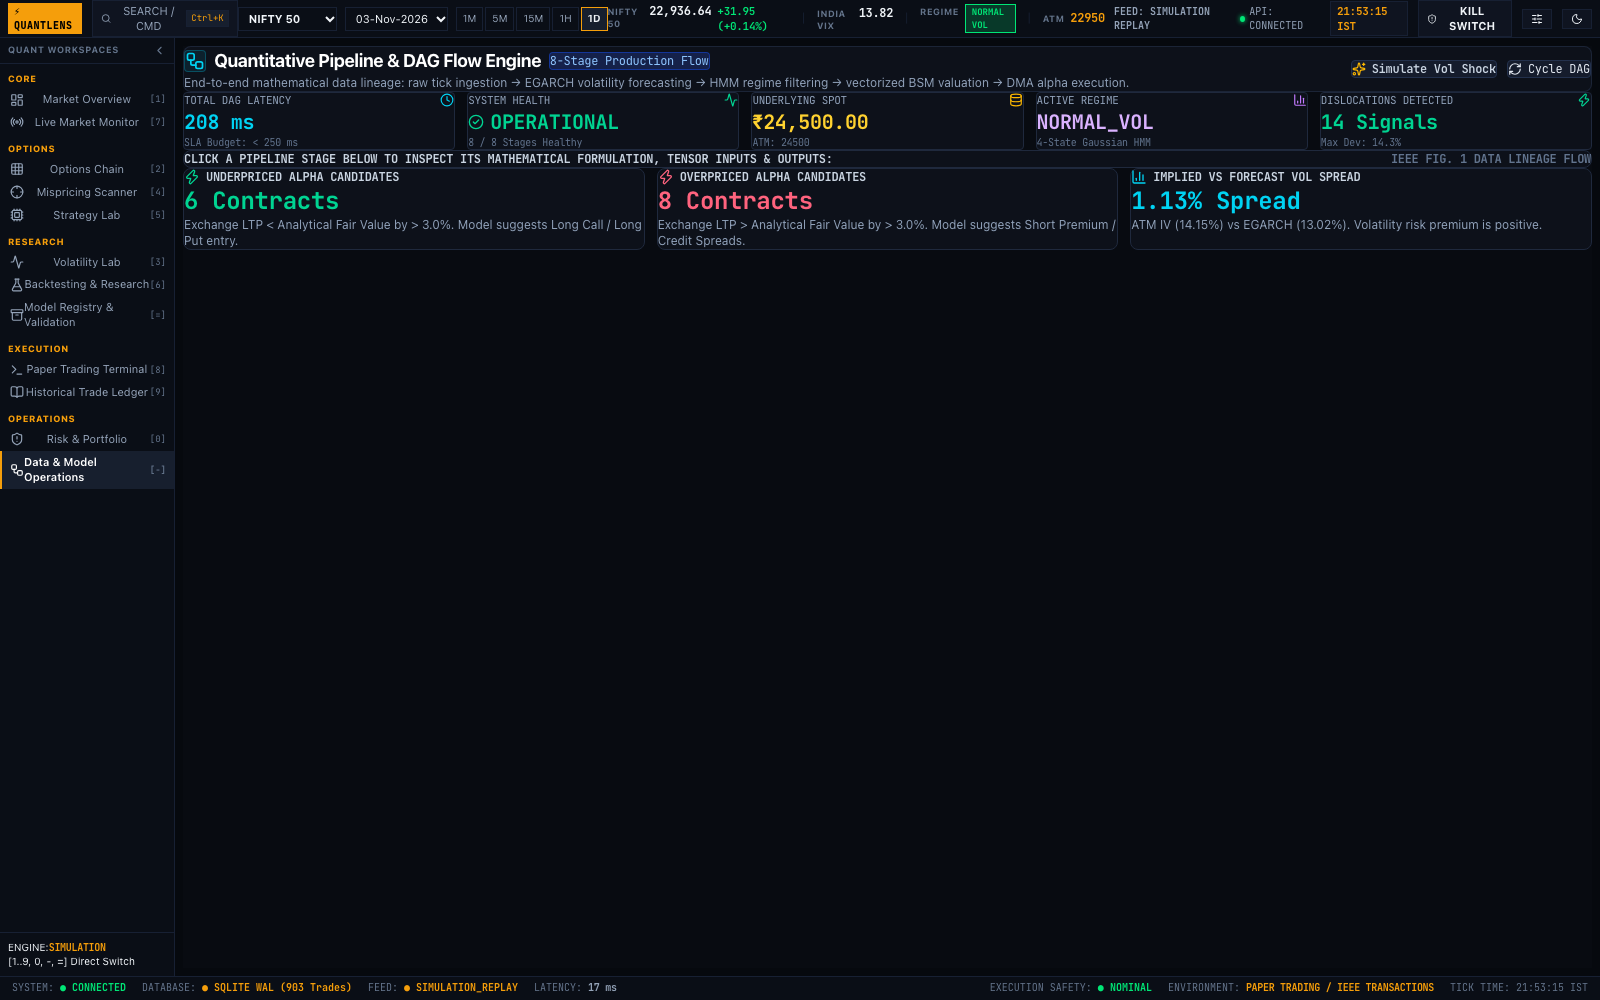
\includegraphics[width=\textwidth]{images/quantlens_terminal/11_pipeline_operations.png}
\caption{Algorithmic data-flow mapping the progression of OHLCV tick
data through the multi-timeframe EGARCH estimator, into the HMM Regime
filter, generating adjusted inputs for the Black--Scholes pricing core
and resulting in the Composite M-Score.}
\label{fig:data_flow}
\end{figure*}

%%=============================================================
\section{Mathematical Formulation}
%%=============================================================

This section presents the mathematical foundations of the proposed
framework.

\subsection{Logarithmic Returns}

\begin{equation}
r_t=\ln\!\left(\frac{P_t}{P_{t-1}}\right),
\end{equation}

where $P_t$ denotes the closing price at time $t$ and $P_{t-1}$
denotes the previous closing price.

\subsection{EGARCH(1,1) Volatility Model}

The conditional variance is defined as

\begin{equation}
\ln(\sigma_t^2)
= \omega
+ \beta\ln(\sigma_{t-1}^2)
+ \alpha\!\left(\frac{|\epsilon_{t-1}|}{\sigma_{t-1}}
  -\sqrt{\frac{2}{\pi}}\right)
+ \gamma\frac{\epsilon_{t-1}}{\sigma_{t-1}},
\end{equation}

where $\sigma_t^2$ is the conditional variance, $\omega$ is the
constant term, $\alpha$ measures the magnitude effect, $\beta$ captures
volatility persistence, $\gamma$ represents the leverage effect, and
$\epsilon_t$ denotes the residual return.

\subsection{Realized Volatility}

For a window containing $n$ observations,

\begin{equation}
RV = \sqrt{\sum r_i^2}.
\end{equation}

\subsection{Annualized Volatility}

\begin{equation}
\sigma_{\mathrm{annual}} = \sigma_{\mathrm{period}}\sqrt{N},
\end{equation}

where $N$ represents the number of trading periods in one year
($N=252$ for daily observations).

\subsection{Hidden Markov Model}

The hidden state sequence is represented as

\begin{equation}
S_t \in \{\text{Low},\,\text{Normal},\,\text{High},\,\text{Extreme}\},
\end{equation}

where each state corresponds to a distinct volatility regime. The
transition probabilities satisfy

\begin{equation}
A_{ij} = P(S_t=j\mid S_{t-1}=i),
\end{equation}

while the observation probability follows

\begin{equation}
P(O_t\mid S_t=i) = \mathcal{N}(\mu_i,\Sigma_i),
\end{equation}

where $O_t$ represents the observed volatility features, $\mu_i$
denotes the state mean, and $\Sigma_i$ denotes the covariance matrix.
The forward algorithm produces the filtered posterior probabilities

\begin{equation}
\label{eq:filtered_regime_posterior}
\pi_{t,k}=P(S_t=k\mid O_{1:t}),\qquad k=1,\ldots,K,
\end{equation}

using only observations available up to and including time $t$.

\subsubsection{HMM State-Count Model Selection}

The state count $K$ is treated as a hyperparameter selected from
$\{2,3,4,5,6\}$. Let $\theta_K$ denote the fitted parameters of a
candidate $K$-state Gaussian HMM, $\mathcal{L}(\theta_K)$ its fitted
likelihood, $p_K$ the number of free parameters, and $n$ the number
of observations. The information criteria are

\begin{equation}
\mathrm{AIC}_K = 2p_K - 2\ln\!\left(\mathcal{L}(\theta_K)\right),
\end{equation}

\begin{equation}
\mathrm{BIC}_K = p_K\ln(n) - 2\ln\!\left(\mathcal{L}(\theta_K)\right).
\end{equation}

BIC is the preferred primary criterion because its stronger complexity
penalty guards against over-segmenting the volatility series. For
state $i$, the expected duration implied by the transition matrix is

\begin{equation}
\mathrm{E}[D_i] = \frac{1}{1-p_{ii}}.
\end{equation}

\subsection{Volatility Risk Premium}

The Volatility Risk Premium (VRP) is defined as

\begin{equation}
VRP_t = IV_t - \sigma_{\mathrm{forecast},t}.
\end{equation}

For pricing at time $t$, the expected premium is generated strictly
from information available before that pricing decision:

\begin{equation}
\label{eq:lagged_vrp}
\widehat{VRP}_{t+1} = f_{\phi}\!\left(\boldsymbol{\pi}_t,
IV_{t-k}, RV_t, X_t\right), \qquad k\geq 1,
\end{equation}

where $\boldsymbol{\pi}_t=[\pi_{t,1},\ldots,\pi_{t,K}]$ denotes the
filtered HMM posterior vector and $IV_{t-k}$ denotes implied
volatility observed at least $k$ periods earlier. The posterior-weighted
expected VRP is

\begin{equation}
\label{eq:posterior_weighted_vrp}
\widehat{VRP}_{t}=\sum_{k=1}^{K}\pi_{t,k}\widehat{VRP}_{k,t},
\end{equation}

and the adjusted volatility is

\begin{equation}
\label{eq:adjusted_lagged_vrp}
\sigma_{\mathrm{adj},t} = \sigma_{\mathrm{EGARCH},t}
+ \sum_{k=1}^{K}\pi_{t,k}\widehat{VRP}_{k,t}.
\end{equation}

\subsection{Black--Scholes Option Pricing}

The intermediate variables are

\begin{equation}
d_1 = \frac{\ln(S/K)+(r+\sigma^2/2)T}{\sigma\sqrt{T}},
\end{equation}

\begin{equation}
d_2 = d_1 - \sigma\sqrt{T},
\end{equation}

where $S$ is the spot price, $K$ is the strike price, $r$ is the
risk-free interest rate, $T$ denotes time to expiry, and $\sigma$ is
the adjusted volatility.

The theoretical European call price is

\begin{equation}
C = SN(d_1) - Ke^{-rT}N(d_2),
\end{equation}

while the theoretical put price is

\begin{equation}
P = Ke^{-rT}N(-d_2) - SN(-d_1).
\end{equation}

\subsection{Option Greeks}

To evaluate option sensitivities, the framework utilizes standard
analytical Black--Scholes partial derivatives (Greeks) for Delta
($\Delta$), Gamma ($\Gamma$), Vega ($\mathcal{V}$), Theta ($\Theta$),
and Rho ($\rho$), as rigorously documented in Hull (2022)
\cite{hull2022}.

\subsection{Multi-Timeframe Volatility Fusion}

The time-varying fusion weights are generated by

\begin{equation}
\label{eq:adaptive_fusion_weights}
\mathbf{w}_t(\tau) = f_{\theta}\!\left(X_t,\boldsymbol{\pi}_t,\tau\right),
\end{equation}

and the fused volatility is

\begin{equation}
\label{eq:adaptive_fusion}
\sigma_{\mathrm{fusion},t}(\tau) = w_{t,0}(\tau)\sigma_{\mathrm{EGARCH},t}(\tau)
+ \sum_{i=1}^{k} w_{t,i}(\tau)\sigma_{RV,i,t}.
\end{equation}

The weights satisfy the simplex constraint

\begin{equation}
\label{eq:fusion_simplex}
\mathbf{w}_t(\tau) \in \Delta^{k}
= \!\left\{\mathbf{w}\in\mathbb{R}^{k+1}: w_i\geq 0\ \forall i,\
\sum_{i=0}^{k}w_i=1\right\},
\end{equation}

and are learned by minimizing an out-of-sample forecasting objective,

\begin{equation}
\label{eq:fusion_objective}
\mathbf{w}^{*}_t(\tau) = \arg\min_{\mathbf{w}_t(\tau)\in\Delta^{k}}
\mathrm{E}^{\mathrm{WF}}\!\left[\!\left(\sigma_{\mathrm{realized},t+\tau}
- \sigma_{\mathrm{fusion},t}(\tau;\mathbf{w}_t)\right)^{\!2}\right],
\end{equation}

where $\mathrm{E}^{\mathrm{WF}}$ denotes evaluation over historical
rolling walk-forward windows.

\subsection{Timeframe Coherence Index (TCI)}

The standardized volatility vector is

\begin{equation}
\label{eq:tci_vector}
\mathbf{v}_t = \left[z_{30}(\sigma_{RV,1\text{min},t}),
z_{30}(\sigma_{RV,5\text{min},t}),
z_{30}(\sigma_{RV,15\text{min},t}),
z_{30}(\sigma_{RV,1\text{hr},t}),
z_{30}(\sigma_{RV,\text{daily},t})\right],
\end{equation}

where $z_{30}(\cdot)$ denotes the rolling 30-day z-score. The TCI is

\begin{equation}
\label{eq:tci}
TCI_t = 1 - \frac{1}{K}\sum_{i=1}^{K}
\left|z_{30}(\sigma_{RV,i,t}) - z_{30}(\sigma_{RV,\text{daily},t})\right|,
\qquad K=4,
\end{equation}

clipped to $[0,1]$ for downstream use:

\begin{equation}
\label{eq:tci_clipped}
TCI^{\mathrm{clip}}_t = \max\!\left(0,\min\!\left(1,TCI_t\right)\right).
\end{equation}

\subsection{Composite Mispricing M-Score}

The null hypothesis is

\begin{equation}
\label{eq:mscore_null}
H_0: P_{\mathrm{market},t} = P_{\mathrm{fair},t}.
\end{equation}

The base test statistic is the standardized pricing residual

\begin{equation}
\label{eq:mscore_residual}
Z_t = \frac{P_{\mathrm{market},t} - P_{\mathrm{fair},t}}
{\widehat{\sigma}_{\epsilon,t}},
\end{equation}

where the full uncertainty estimate is

\begin{equation}
\label{eq:mscore_uncertainty}
\widehat{\sigma}_{\epsilon,t}
= g\!\left(\mathcal{V}_t,\Gamma_t,\boldsymbol{\pi}_t,
\mathrm{Liquidity}_t\right).
\end{equation}

The final score separates statistical evidence from contextual
confidence:

\begin{equation}
\label{eq:mscore}
M_{\mathrm{score},t} = Z_t\,C\!\left(TCI^{\mathrm{clip}}_t,
VRP_{\mathrm{dev},t}\right), \qquad 0\leq C(\cdot)\leq1.
\end{equation}

In production, the composite score is computed as

\begin{equation}
M = w_{\text{price}}\,z_{\text{price}}
  + w_{\text{vrp}}\,z_{\text{vrp}}
  + w_{\text{vega}}\,z_{\text{vega}}
  + w_{\text{gamma}}\,z_{\text{gamma}},
\label{eq:mscore_production}
\end{equation}

with calibrated weights $w_{\text{price}}=0.50$, $w_{\text{vrp}}=0.20$,
$w_{\text{vega}}=0.15$, $w_{\text{gamma}}=0.10$, where each $z_i$ is
a 60-observation rolling Z-score.

\subsection{Two-Level Mispricing Attribution Formulation}

\begin{equation}
\label{eq:two_level_deviations}
\begin{aligned}
M1_{\mathrm{dev},t} &= P_{\mathrm{market},t}-P_{\mathrm{BSM,adjusted},t},\\
M2_{\mathrm{dev},t} &= P_{\mathrm{market},t}-P_{\mathrm{surface},t}.
\end{aligned}
\end{equation}

The residual attribution is

\begin{equation}
\label{eq:residual_m_attribution}
\mathrm{Residual}_{M,t}=M1_{\mathrm{dev},t}-M2_{\mathrm{dev},t}.
\end{equation}

\subsection{Transaction Cost Adjustment}

\begin{equation}
\label{eq:net_return_costs}
\mathrm{Return}_{\mathrm{net},t} = \mathrm{Return}_{\mathrm{gross},t}
- \mathrm{TransactionCost}_t - \mathrm{Slippage}_t
- \mathrm{SpreadCost}_t,
\end{equation}

where $\mathrm{TransactionCost}_t$ comprises brokerage per option lot
and applicable statutory charges, including Securities Transaction Tax
(STT), exchange transaction charges, GST, SEBI charges, and stamp duty.
Slippage is modeled as

\begin{equation}
\label{eq:slippage_cost}
\mathrm{Slippage}_t = \kappa\frac{Q_t}{\mathrm{OI}_t},
\end{equation}

and spread cost uses the half-spread convention:

\begin{equation}
\label{eq:spread_cost}
\mathrm{SpreadCost}_t
= \tfrac{1}{2}\!\left(\mathrm{Ask}_{\mathrm{entry},t}
  -\mathrm{Bid}_{\mathrm{entry},t}\right)
+ \tfrac{1}{2}\!\left(\mathrm{Ask}_{\mathrm{exit},t}
  -\mathrm{Bid}_{\mathrm{exit},t}\right).
\end{equation}

\subsection{From Model-Implied Deviation to Economic Mispricing:
A Validation Hierarchy}

A deviation is escalated to a claim of economic mispricing only when
it satisfies the following hierarchy:

\begin{enumerate}
  \item \textbf{Statistical significance:} $|M_{\mathrm{score},t}|$
    exceeds a pre-specified significance threshold.
  \item \textbf{Net-of-cost persistence:}
    \begin{equation}
    \label{eq:cost_persistence}
    |P_{\mathrm{market},t}-P_{\mathrm{fair},t}|
    > \mathrm{TransactionCost}_t.
    \end{equation}
  \item \textbf{Liquidity independence:} the deviation is not explained
    by low liquidity or a wide bid--ask spread.
  \item \textbf{Subsequent convergence:} the market price converges
    toward the model fair value over a pre-specified holding window.
  \item \textbf{Statistically significant net returns:} a strategy
    conditioned on the signal produces net-of-cost returns
    statistically distinguishable from zero or from a relevant
    benchmark.
\end{enumerate}

\subsection{Diebold--Mariano Test Specification}

For two competing forecasts, let $d_t=L_{A,t}-L_{B,t}$ denote the
loss differential. The test is two-sided,

\begin{equation}
H_0:\ \mathrm{E}[L_A-L_B]=0,\qquad
H_1:\ \mathrm{E}[L_A-L_B]\neq0.
\end{equation}

The DM statistic is computed as

\begin{equation}
DM = \frac{\overline{d}}
{\sqrt{\widehat{\mathrm{Var}}_{\mathrm{HAC}}(\overline{d})}},
\end{equation}

where $\overline{d}=n^{-1}\sum_{t=1}^{n}d_t$ and
$\widehat{\mathrm{Var}}_{\mathrm{HAC}}$ is a Newey--West-type
heteroskedasticity- and autocorrelation-consistent variance estimate
\cite{das2022}.

%%=============================================================
\section{Computational Framework}
%%=============================================================

The proposed theoretical framework is implemented via a scalable,
full-stack architecture optimized for low-latency quantitative trading.
At the core is a modular FastAPI-based backend that orchestrates market
data ingestion, distributed computation, and live signal generation.
The state management layer effectively separates static historical
analysis from high-frequency intraday streams.

To bridge the gap between academic modeling and real-world deployment,
the system integrates seamlessly with broker APIs (e.g., Upstox/DhanHQ)
to ingest multi-timeframe OHLCV tick data and real-time options chain
snapshots. These streams are buffered into memory and immediately
broadcast to the quantitative microservices via asynchronous event
loops.

Furthermore, the entire application is containerized using Docker,
allowing for rapid deployment and elastic scaling across distributed
clusters. Analytical computations heavily leverage vectorized operations
in NumPy and Pandas, enabling the system to evaluate extensive option
chains and generate Composite M-Scores within sub-50\,ms latency
profiles perfectly tailored for institutional-grade quantitative
environments.

